\documentclass[12pt,a4paper]{article}
\usepackage{helvet}
\renewcommand{\familydefault}{\sfdefault}
\usepackage[T1]{fontenc}
% \usepackage[croatian]{babel}
\usepackage[utf8]{inputenc}
\usepackage{amsmath}
\usepackage{amsfonts}
\usepackage{amssymb}
\usepackage{graphicx}
\usepackage{fancyhdr}
\usepackage{setspace}
\usepackage{color}
\usepackage[hidelinks, breaklinks]{hyperref}
\usepackage[nottoc]{tocbibind}
\usepackage{secdot}


\graphicspath{ {./images/} }
\date{}

\renewcommand*\contentsname{Sadržaj}
\renewcommand{\listfigurename}{Slike}
\renewcommand{\listtablename}{Tablice}
\renewcommand{\figurename}{Slika}
\renewcommand{\tablename}{Tablica}
\setcounter{secnumdepth}{3}
\setcounter{tocdepth}{5}

\definecolor{m}{RGB}{31, 189, 191}
\definecolor{o}{RGB}{255, 122, 13}
\definecolor{p}{RGB}{195, 0, 255}

\newcommand{\collegeName}{TEHNIČKO VELEUČILIŠTE U ZAGREBU}
\newcommand{\smjer}{STRUČNI STUDIJ RAČUNARSTVA}
\newcommand{\radTittle}{Raspberry pie sigurnosna kamera i IOT implikacije}
\newcommand{\radNumber}{}
\newcommand{\paraBreak}{\\[0.5cm]}
\newcommand{\myparagraph}[1]{\paragraph{#1}\mbox{}\\[6pt]}

\newcommand{\foreign}[1]{\emph{#1}}
\newcommand{\keyword}[2][m]{\textcolor{#1}{#2}}

\begin{document}

\begin{center} \obeylines
  \setstretch{2}
  {\large \textbf{\collegeName}}
  {\normalsize \textbf{\smjer}}
\end{center}
\begin{center} \obeylines
  \setstretch{1.6}
  \vspace{\fill}
    Domagoj Živanović 
    {\Large \textbf{\radTittle}}
    \item ZAVRŠNI RAD br. \radNumber
  \vspace*{\fill}
  Zagreb, Srpanj, 2020.
\end{center}

\thispagestyle{empty}

\clearpage

\begin{center} \obeylines
  \setstretch{2}
  {\large \textbf{\collegeName}}
  {\normalsize \textbf{\smjer}}
\end{center}
\begin{center} \obeylines
  \setstretch{1.75}
  \vspace{\fill}
      Domagoj Živanović
      JMBAG: 0036483209
    {\Large \textbf{\radTittle}}
    ZAVRŠNI RAD br. \radNumber
  \vspace*{\fill}
  Zagreb, Srpanj, 2020.
\end{center}

\thispagestyle{empty}

\clearpage


\tableofcontents
\clearpage
\listoftables
\listoffigures

\section{Sažetak}
Ovaj rad bavi se implementacijom sigurnosne kamere koristeći raspberry pi s kamera modulom, 
te prijenosom videa iste raznim klijentima.
\paraBreak
Projekt se sastoji od 3 glavna sustava \textbf{Transkoder}, \textbf{Server}, \textbf{Klijenti}
\paraBreak
Kroz rad su opisana sva 3 dijela sustava te njihove međusobne interakcije, funkcionalnosti te dizajn.
\paraBreak
Glavni cilj rada je implementirati kompletni sustav za nadzor kojem se može pristupiti kroz velik niz klijenata kao što su web browser, mobitel itd.

\section{Uvod}
Video nadzor se danas uvelike koristi u velikom broju raznih područja kao na primjer sigurnost, medicina, transport
i brojni drugi.
\paraBreak
Zbog naglog usvajanja interneta proteklih godina, većina nadzornih sustava, takozvani "pametni" uređaji, oslanjaju se
na komunikaciju putem istog. \\
Tradicionalni nadzorni sustav sastoji se od naravno od kamere, neke vrste prijenosnog kabla koji povezuje kameru sa
računalom te video nadzorne platforme odnosno aplikacijom. Ovaj radi se primarno bavi implementacijom aplikacijskog djela a 
za sklopovski dio koristi Raspberry pi platformu.
\paraBreak
Video nadzor možemo generalno podijeliti na dvije vrste, pasivni nadzor i nadzor u realnom vremenu. \\
Kod pasivnog nadzora nije moguće u bilo kojem trenutku vidjeti prikaz kamere, video se sprema na neku vrstu spremišta, bilo
lokalno kao tvrdi disk ili 
\foreign{cloud}
\footnote
{
  Aplikacije ili softver uvijek dostupni putem interneta, na poslužiteljima treće strane, obično se iznajmljuju na neki ne nužno
  određen period vremena 
}
rješenje. \\
Nadzor u realnom vremenu kao što i ime sugerira omogućuje pregled u bilo kojem trenutku, ali najčešće i pohranjuje
video na isti način kao i pasivni. \\
Implementacija ovog rada spada pod nadzor u realnom vremenu, ali na nikakav način ne pohranjuje snimani video, zbog pre velikih
troškova koje takva pohrana nosi. 
\paraBreak
Svrhe ovakvih pametnih nadzora su brojne, ali osim očitih, zbog velikog napretka računalnih mreža, procesiranja digitalnih
slika i načina prijenosa podataka relativno je lako doći do robusnih i pametnih implementacija koje koriste strojno učenje
za prepoznavanje događaja koje je odredio korisnik. Takvi nadzorni sustavi imaju ogroman potencijal i integraciju sa virtualno
bilo kojim uređajem koji ima pristup internetu. Kao demonstraciju u sklopu ovog rada implementiran je poslužitelj
koji je sposoban prenositi nadzorni video velikom broju uređaja pod uvjetom da su spojeni na internet.

\pagebreak
\subsection{Raspberry pi}
Raspberry pi je serija malih \foreign{single-board \footnote{Računalo u potpunosti izgrađeno na jednoj pločici}} 
računala široko korištenih u svrhe eksperimentalnih projekata. \cite{rPiBook}
\paraBreak
Idealan je za tu upotrebu zbog privlačne cijene i odlične portabilnosti te jako male potrošnje struje.
\paraBreak
Za ovaj rad je odabran zbog osim navedenih razloga još i radi ogromnog izbora eksternih modula, specifično službenog kamera modula
koji služi kao baza cijelog projekta.

\begin{figure}[ht]
  \centering
  \begin{subfigure}{.5\textwidth}
    \centering
    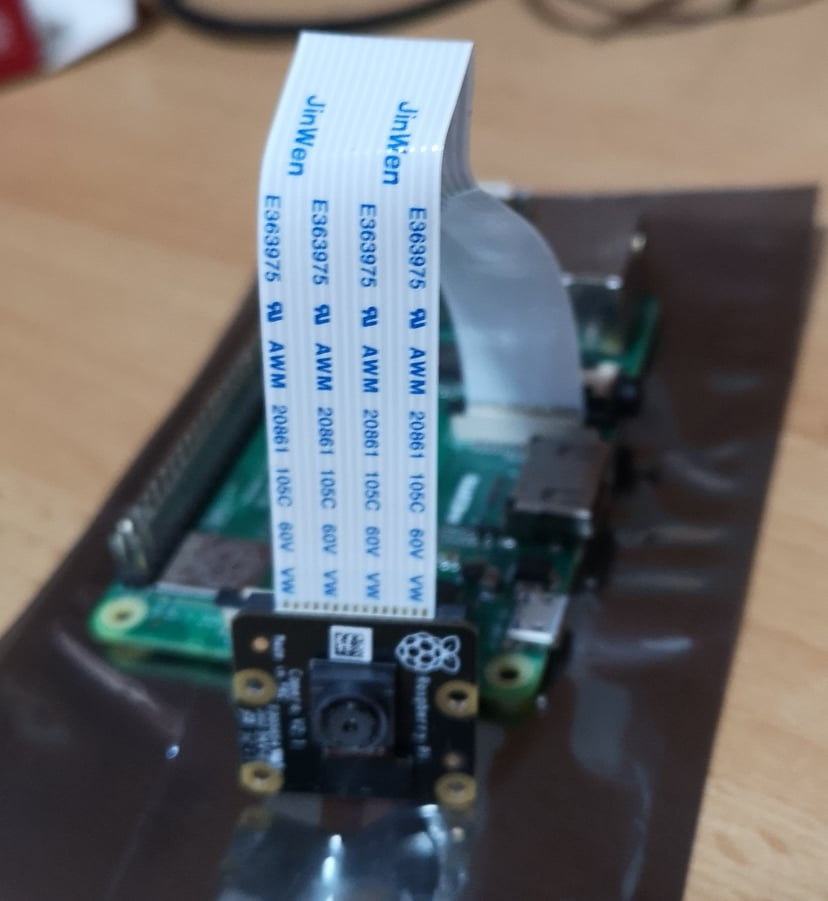
\includegraphics[width=0.95\textwidth]{raspberyy-pi-camera.jpg}
    \caption{Kamera modul}
  \end{subfigure}%
  \begin{subfigure}{.5\textwidth}
    \centering
    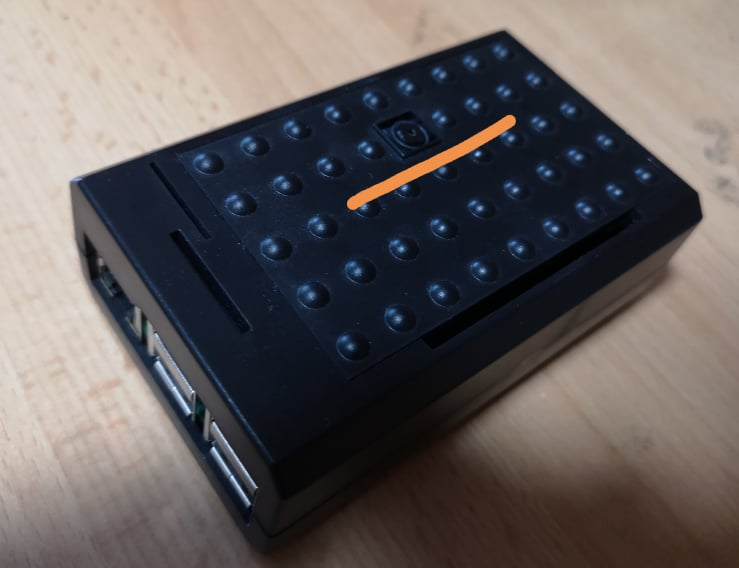
\includegraphics[height=7.6cm, width=0.95\textwidth]{raspberyy-pie-in-box.jpg}
    \caption{Kutija sa otvorom za leću kamere}
  \end{subfigure}%
  \caption{Raspberry pi dodaci}
\end{figure}

\clearpage
\subsection{Biblioteka za obradu videa} \label{sec:ffmpeg}
  \foreign{FFmpeg} je 
  \footnote
  {
    Projekti koji otvoreno dozvoljavaju korištenje istih ovisno o licensama, te koji imaju javno dostupan izvorni kod
    i najčešće se oslanjaju na zajednicu programera na daljnjem razvoju.
  }
  {\foreign{open-source}} 
  projekt koji se sastoji od mnoštva biblioteka za manipuliranje videom, audiom i ostalom multimedijom.
  \cite{ffmpegBook}
\paraBreak
Najveća primjena mu je u transkodiranju, editiranju, skaliranju i raznim efektima videa.
\paraBreak
Najbitnije biblioteke iz FFmpeg-a koje se koriste u ovom radu su \cite{ffmpegDocs}
\begin{itemize}
  \item libavcodec - audio/video kodek biblioteka
  \item libavformat - audio/video kontejner \hyperref[sct:mux]{\foreign{}{mux}} i \hyperref[sct:demux]{\foreign{}{demux}} biblioteka
  \item libavdevice - biblioteka za dohvaćanje i rad dostupnim multimedija uređajima
  \item libswscale - biblioteka za manipulaciju i skaliranje slika videa
\end{itemize}
Koristi se u mnogim popularnim projektima kao što su Google Chrome, VLC Player, YouTube, Blender, HandBrake, Kodi, Plex. \cite{ffmpegBook}

\section{Pregled}

\subsection{Arhitektura}
Cijeli sustav je rastavljen u 3 glavna dijela
\begin{itemize}
  \item Transkoder
  \item Poslužitelj
  \item Klijenti
\end{itemize}
Način međusobne interakcije između ova tri dijela sustava je jasno vidljiv na slici \ref{pic:flow_diagram}
\paragraph{Transkoder}
je zadužen za primanje podataka od kamere i transformiranje istih u format koji je odgovarajuć za najveći broj klijenata, 
te slanje u realnom vremenu na poslužitelj putem TCP-a.
\paragraph{Poslužitelj}
je zadužen za autentifikaciju klijenata te prosljeđivanje paketa koje prima od Transkodera putem HTTP-a.
\paragraph{Klijenti}
nakon što se autoriziraju s poslužiteljom, primaju pakete videa putem HTTP-a te ih prikazuju korisniku.
\begin{figure}[h]
  \centering
  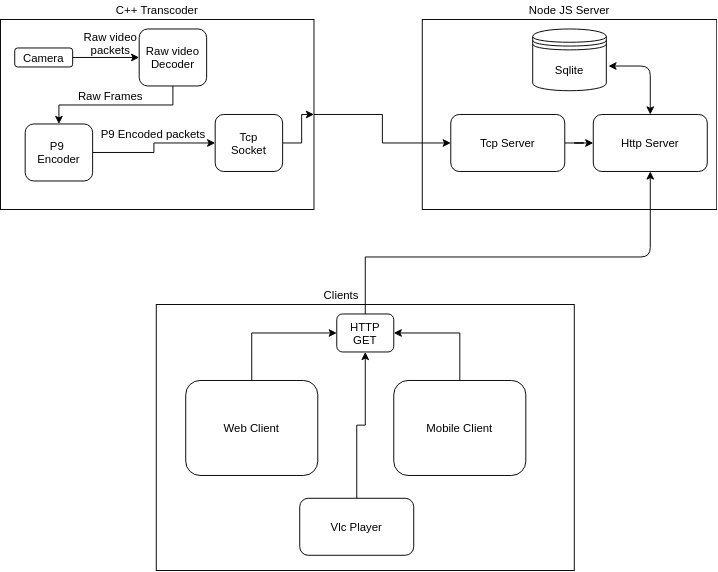
\includegraphics[height=9cm, width=\textwidth]{flow-diagram.png}
  \caption{Flow diagram sustava}
  \label{pic:flow_diagram}
\end{figure}

\clearpage
\subsection{Tehnologije}

\subsubsection{Programski jezik C++}
C++ je odabran za implementaciju transkodera, primarno zato što su FFMpeg biblioteke napisane u jeziku C 
s kojim se C++ vrlo jednostavno integrira ali i zbog manjka memorije Raspberry pi-a i teške prirode posla kojeg obavlja
u smislu potrebne snage procesora zbog čega je bitno imati jezik koji se prevodi u nativni kod ovisno o platformi te koji
je memorijski učinkovit. \cite{bStrou}

\subsubsection{Okruženje Node JS}
Node JS je \foreign{open-source cross-platform runtime} za JavaScript. \\
Omogućuje pisanje poslužiteljskog koda u jeziku JavaScript. \cite{nodeBook}
\paraBreak
Idealan je za poslužitelja ovog projekta zbog svog \foreign{event-driven} asinkronog pristupa.
Priroda posla koju poslužitelj obavlja ne zahtijeva veliku procesnu snagu nego mogućnost serviranja velikog broja zahtjeva
paralelno, \foreign{Node JS} se upravo u takvom tipu posla ističe. \cite{nodeBook}

\subsubsection{Biblioteka React JS}
React JS je \foreign{open-source} JavaScript biblioteka za izradu web aplikacija.
\paraBreak
Izabran je za implementaciju primjera web klijenta jer je klijent zamišljen da bude dinamična web aplikacija a ne statička
stranica, s potencijalno velikim brojem odlika. \cite{reactBook}
\paraBreak

\clearpage
\subsection{Video} \label{sec:video}
Video je ništa drugo nego niz slika koje se mijenjaju određenom frekvencijom, u slučaju filmova naj češće 24 slika 
po sekundi (24 FPS). \cite{ffmpegBook}

\subsubsection{Slika} \label{sec:slika}
Slika opisuje dekodirane čiste podatke videa. \\
U kontekstu enkodiranja postoje 3 glavne vrste \begin{itemize}
  \item \textbf{I} Slika - kompletna slika
  \item \textbf{P} Slika - predviđena slika, sadrži samo promjene od prethodne slike
  \item \textbf{B} Slika - slično kao i P, sadrži samo promjene ali ne samo od prethodne nego potencijalno i sljedeće 
  slike, te tako sačuva još više mjesta
\end{itemize}

\myparagraph{P i B Slike}
\foreign{P} i \foreign{B} slike su jedan od načina kojim enkoderi smanjuju finalnu veličinu datoteke, 
primjerice zamislimo kameru koja snima promet po noći,
većina slika tog videa će biti jako slična sve dok se ne pojavi auto, enkoder zato ne mora sve informacije spremati u svaku P sliku
već samo onaj dio slike gdje se pojavio auto dok ostatak uzme iz prethodne.
\paraBreak
To funkcionira tako da se uzme proizvoljan interval \foreign{I} slika, još poznatim kao \foreign{keyframe} recimo 
svakih 15 slika, tada enkoder svaku 15-tu sliku enkodira u potpunosti dok ostale enkodira kao \foreign{P} ili \foreign{B} slike.
\\
Što je interval I slika veći to će video u konačnici biti manji.
\paraBreak
Bitno je za znati da se na \foreign{P} i \foreign{B} slike ne može tražiti (\foreign{seek}), jer te slike sadrže samo frakciju podataka potrebnih
da se izgradi kompletna slika, recimo da imamo video koji se vrti 30 slika u sekundi te enkodiramo \foreign{I} sliku 
svakih 10 sekundi ili 900 slika, tada bi video bilo moguće premotavati naprijed ili nazad samo u intervalima od 10 sekundi.
\paraBreak
Stoga ako je bitno da se video može premotavati u malim intervalima mora se postaviti Interval \foreign{I} 
slika na što manju vrijednost.

\subsubsection{Način zapisa slike} \label{sec:pixelformat}
Piksel format je format ili način na koji je svaki pojedinačni piksel slike zapisan odnosno opisuje kako su podaci o boji
svakog piksela enkodirani. Primjerice piksel format \foreign{24 bit RGB} još poznat kao \foreign{RGB888} 
zauzima 3 bajta po pikselu, jedan bajt za svaki od kanala.
\paraBreak
Enkoderi preferiraju \textbf{planarne} piksel formate, primjerice h264 enkoder podržava samo \foreign{yuv420p} piksel format, što
znači da se za enkodiranje tipičnog videa mora raditi pretvorba iz RGB piksel formata u yuv420p. \\
Jedan od razloga je memorijska efikasnost, primjerice \foreign{RGB888} piksel format zauzima 3 bajta po pikselu dok
yuv420p zauzima 6 bajta svaka 4 piksela. \cite{ffmpegBook}

\paragraph{Planaran} \label{sec:planar} piksel format znaci da predstavlja boje piksela kroz nekoliko ravnina ili 
ploha, uglavnom 3 ravnine. \\
Svaki bit ovih ravnina predstavlja dio piksela slike. To je korisno jer se podaci o pikselu više ne nalaze u jednom 
neprekidnom polju odnosno istoj lokaciji u memoriji, nego su razdvojeni na više polja.

\subsubsection{Kontejner} \label{sec:container}
Kontejner je jedna datoteka koja sadrži sve tokove kao što su video, audio i titlovi.\\
Još sadrži sve metapodatke kao što su rezolucija videa, FPS, autor, kodek itd. Po tim 
podacima \hyperref[sct:videoPlayer]{\foreign{video player}}-i znaju korektno prikazati sliku i zvuk. \cite{ffmpegBook}
\\
Primjeri nekih kontejnera su:
\begin{itemize}
  \item MPEG-4
  \item Matroska
  \item QuickTime/MP4
  \item WebM
  \item WAW
\end{itemize}

\subsubsection{Kodek} \label{sec:codec}
Kodek je program (ili sklopovlje) koji služi za kompresiju ili dekompresiju videa. \\
Pretvara ne kompresiran (\foreign{Raw}) video u kompresiran i obratno. \\
Ako je riječ o kompresiranju onda je to enkoder, inače dekoder. \cite{ffmpegBook}
\paraBreak
Proces kompresiranja je tipično gubitačan (\foreign{lossy}) što znači da kompresirani video ne sadrži sve informacije kao i original
što rezultira u lošijoj kvaliteti videa i nakon kompresije više nije moguće u potpunosti rekonstruirati original. \cite{ffmpegBook}
\paraBreak
Problem kod videa je veličina, recimo da imamo video rezolucije 1920 x 1080 koji se vrti na 24 slika u sekundi, i da 
koristimo RGB piksel format što znači da nam trebaju 3 bajta po pikselu za enkodiranje boje te da traje 30 minuta 
(trećina ili manje prosječnog filma) \\
Veličina takvog videa bez enkodiranja bila bi \textbf{268.7 GB} \label{sec:size_problem} \cite{ffmpegBook}
\paraBreak
Upravo iz tog razloga moramo imati kodek.

\subsubsection{Podržanost kodeka i kontejnera u raznim preglednicima}
Za živi prijenos postoje 3 naj bolje opcije što se tiče podržanosti \cite{appleCodec} \cite{androidCodec} \cite{canIUse}

\begin{center}
  \begin{table}[h]
    \begin{tabular}{|c|c|c|c|}
      \hline
      & vp8/9 + webm & h264+mp4/DASH & h264 + mkv \\
      \hline
      Chrome & x & x & - \\
      Firefox & x & x & - \\
      Safari & - & x & - \\
      Edge & vp8 & x & - \\
      IOS (Svi preglednici) & - & x & - \\
      Android (Chrome) & x & x & - \\
      \hline
    \end{tabular}
    \caption[Podržanost kodeka i kontejnera u raznim preglednicima]
    {Podržanost kodeka i kontejnera u raznim preglednicima \cite{appleCodec} \cite{androidCodec} \cite{canIUse}}
\end{table}

\end{center}

\myparagraph{Kodek h264 i kontejner rtmp}
H264 je jedan od starijih kodeka i kao takav podržan je na skoro svim uređajima.
Nudi dobar balans kvalitete i brzine. \cite{h264Book}
\paraBreak
Rtmp kontejner je jedan od naj korištenijih kontejnera za živi prijenos, jedan od korisnika je Twitch.tv \\
Problem ovog kontejnera je sto je vlasnik Adobe i nije besplatan, uz to nije podržan nativno u HTML5 video elementu.

\myparagraph{Kodek h264 i kontejner mp4}
U teoriji odlična kombinacija jer je mp4 kontejner podržan virtualno svugdje.
\paraBreak
Nažalost mp4 ne podržava živi prijenos jer mora unaprijed znati točnu duljinu videa što kod živog prijenosa nije moguće. \\
Rješenje je MPEG-DASH (Dynamic Adaptive Streaming over HTTP). Proces razdvajanja videa u manje cjeline s poznatom veličinom.

\myparagraph{Kodek vp8/9 i kontejner webm}
Ovu kombinaciju kodeka i kontejnera je implementirao Google, želeći izbjeći troškove licenci za 264/5 kodek. \\
Glavna snaga mu je odlična kompatibilnost s nativnim HTML 5 video elementom koji je standard u većini preglednika \cite{ffmpegBook}
\paraBreak
Osim toga u usporedbi s puno starijim h264 kodekom, pruža bolju latenciju i kvalitetu slike, pogotovo 
na nižim \hyperref[sct:bitRate]{\foreign{bit rate}} a uz to je i efikasniji što se tiče resursa. \cite{ffmpegBook}
\paraBreak
Najveći problem mu je Apple koji odbija implementirati ovu kombinaciju u Safariju i IOS operativnom sustavu. \\
Također za razliku od mp4 kontejnera webm nije kodek agnostičan, to jest može se kombinirati samo sa vp8 ili vp9 kodecima. \cite{ffmpegBook}
\paraBreak
Upravo ova kombinacija je odabrana u ovom radu zbog svoje relativne jednostavnosti i dobre podržanosti.

\section{Implementacija}

\subsection{Transkoder}
Opis transkoder implementacije
\clearpage

\subsubsection{FFmpeg strukture}
Biblioteka FFmpeg dolazi sa ogromnim brojem struktura, velik dio od kojih nema veze sa samom manipulacijom videa,
u ovom poglavlju su opisane glavne strukture koji su korisne u tu svrhu

\myparagraph{AVInputFormat}
Struktura \keyword{AVInputFormat} 

\myparagraph{AVFormatContext}

\myparagraph{AVStream}

\myparagraph{AVCodec}

\myparagraph{AVCodecContext}

\myparagraph{AVIOContext}

\myparagraph{AVFrame}

\myparagraph{AVPacket}

\myparagraph{SwsContext}

\myparagraph{AVRational}

\myparagraph{AVDictionary}

\clearpage
\subsubsection{Konfiguracija}

\subsubsection{Wrapperi oko FFmpeg struktura}

\subsubsection{Pristup kameri}

\subsubsection{Čitanje paketa iz kamere}

\subsubsection{Dekodiranje paketa}

\subsubsection{Enkodiranje slika}

\subsubsection{Slanje enkodiranih paketa kroz mrežu}


\clearpage
\subsection{Poslužitelj}\label{sec:http_api}
Poslužitelj predstavlja vezu između transkodera\footnote{Potencijalno nekoliko njih u slučaju više kamera} odnosno same 
kamere i klijenata.
\paraBreak
Glavni posao mu je primanje videa od transkodera i preusmjeravanje istog putem HTTP-a autentificiranim klijentima.
\footnote{Primjer klijenta je web preglednik ili mobilna aplikacija}
\subsubsection{Autentifikacija}
Autentifikacija je implementirana pomoću \foreign{JSON Web Tokena} ili \foreign{JWT}
\myparagraph{JWT} \label{sec:jwt}
\foreign{JWT} je kompaktan, siguran način reprezentiranja podataka, kao JSON string, koji se mogu
prenijeti između dvije partije.
\paraBreak
Omogućuje digitalno potpisivanje samog tokena s tajnim ključem ili \foreign{MAC} poznatim samo izdavačkoj 
strani (poslužitelju). Potpis osigurava da se sadržaj tokena ne može promijeniti bez da se invalidira potpis. \cite{JWT}
\paraBreak
Sam token se sastoji od tri dijela:
\begin{itemize}
  \item Header - ili zaglavlje opisuje koji se algoritam koristio tijekom enkodiranja
  \item Podaci
  \item Digitalni potpis ako ga ima
\end{itemize}
Token može bilo tko dekodirati i vidjeti podatke koji se u njemu nalaze, ali se ne može promijeniti bez invalidiranja
potpisa. \cite{JWT}
\paraBreak
Tipičan tijek razgovora između poslužitelja i klijenta koristeći ovaj način autentifikacije izgleda ovako:
\begin{enumerate}
  \item Klijent se putem forme prijavljuje slanjem korisničkog imena i lozinke.
  \item Poslužitelj provjerava poslane podatke i ako odgovaraju šalje kao odgovor JWT token potpisan tajnim \\
  ključem koji sadrži jedinstveni identifikator klijenta.
  \item Klijent token trajno pohranjuje i u \foreign{Authorization} 
    \footnote{Ne mora nužno biti \foreign{Authorization} zaglavlje, to je samo konvencija} 
    zaglavlju svakog sljedećeg zahtjeva
    šalje token.
  \item Poslužitelj vidi da je token prisutan u zaglavlju te ga verificira vlastitim potpisom pa dekodira i izvlači iz 
    njega jedinstveni identifikator klijenta po kojem onda zna točno o kojem klijentu je riječ. \\
    Poslužitelj može biti siguran da klijent nije mogao sam promijeniti taj token, primjerice vlastitu rolu u 
    administratorsku jer bi to invalidiralo potpis.
\end{enumerate}
Ovaj način autentifikacije je privlačan jer za razliku od sesija ne ovisi o bazi, što rezultira u puno bržoj 
autentifikaciji, mana mu je što je teško invalidirati tokene nakon što su izdani. \cite{JWT}

\begin{figure}[h]
  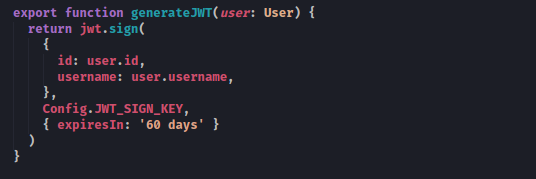
\includegraphics[width=\textwidth]{generate_jwt.png}
  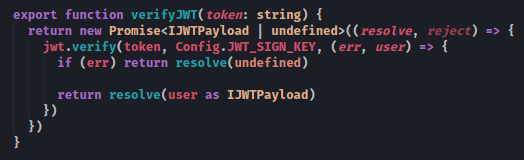
\includegraphics[width=\textwidth]{verify_jwt.png}
  \caption{Generiranje i verificiranje tokena}
\end{figure}

\myparagraph{Baza}
Za pohranu korisnika koristi se \foreign{SQLite} baza podataka.
\paraBreak
Ova baza je odabrana primarno zbog svoje jednostavnosti, naime za razliku od ostalih baza koje funkcioniraju na
klijent-poslužitelj modelu, ova baza je kompletno ugrađena u jednu datoteku. \cite{SQLite} \\
Zbog jednostavnosti i malog broja entiteta poslužitelja ova baza je idealno rješenje.
\paraBreak
Entiteti u bazi predstavljeni su u obliku klasa, kroz \foreign{ORM} (engl. Object-Relational Mapping).
\foreign{ORM} je tehnika manipulacije i ispitivanja baze pomoču objektno orijentirane paradigme, točnije svaka tablica
baze predstavljena je jednim objektom ili klasom koja pomoču raznih metoda generira \foreign{SQL} upite prema bazi.
Primjer jedne takve klase je prikazan na slici \ref{pic:orm-entity}.
\\
Iz sigurnosnih razloga lozinka korisnika je \footnote
{
  Heširanje (engl. Hashing) je proces transformiranja teksta u jedinstveni oblik iz kojega više nije moguče doći
  do originalnog teksta. Heširanje dvaju istih tekstova uvijek mora rezultirati istim vrijednostima.
}{heširana} 
\foreign{Bcrypt} algoritmom. 
U slučaju komprimiranja baze na poslužitelju napadač nemože iz tablice korisnika pročitati lozinke kao što se vidi
na slici \ref{pic:hashed_password}.

\begin{figure}[h]
  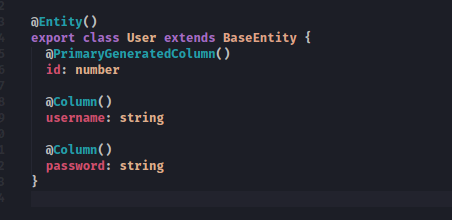
\includegraphics[width=\textwidth]{user_entity.png}
  \caption{User entitet koji predstavlja tablicu u bazi}
  \label{pic:orm-entity}
\end{figure}

\begin{figure}[h]
  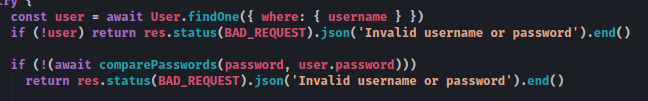
\includegraphics[width=\textwidth]{get_user.png}
  \caption{Dohvaćanje korisnika iz baze i provjera lozinke}
\end{figure}

\begin{figure}[h]
  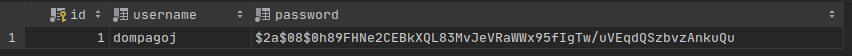
\includegraphics[width=\textwidth]{user_table.png}
  \caption{Tablica korisnika u bazi}
  \label{pic:hashed_password}
\end{figure}

\clearpage
\subsubsection{Komunikacija sa transkoderom} \label{sec:http}
Primarni način kojim poslužitelj komunicira sa transkoderom je TCP (\foreign{Transmission Control Protocol}) protokol. \\
Jedan glavnih i naj zastupljenijih protokola weba povrh kojeg je HTTP protokol implementiran. \cite{webProtocols}
\paraBreak
Nudi pouzdanu vezu u kojoj se za razliku od UDP protokola, primljeni paketi provjeravaju za redoslijed, odnosno TCP
garantira da su svi primljeni paketi stigli istim redoslijedom kojim su i poslani, što je u slučaju video prijenosa jako bitno. \\
\paraBreak
TCP je baziran na konekcijama odnosno veza između klijenta i poslužitelja je uspostavljena prije nego se paketi mogu slati, ovo je
glavni razlog zašto je odabran umjesto UDP protokola koji nudi bolje performanse. Naime jedan od ciljeva je imati
podršku za više kamera odnosno traskodera, što je s TCP-om trivijalno za implementirati, dok bi se s UDP-om moralo
implementirati vlastiti sustav identifikacije svakog paketa.
\paraBreak
Klasa \keyword{StreamingClients} predstavlja listu svih spojenih transkodera odnosno kamera, sadrži metode:
\begin{itemize} \label{sec:sreaming_clients}
  \item \keyword[o]{addClient} - dodaje novog klijenta
  \item \keyword[o]{removeClient} - briše klijenta
  \item \keyword[o]{getClient} - dohvaća klijenta
  \item \keyword[o]{getClients} - vrača listu svih klijenata
\end{itemize}
Privatno polje \keyword[p]{clients} je mapa svih klijenata kojoj je ključ jedinstveni identifikator klijenta, dok
je vrijednost klasa \keyword{CameraStream}. Ona sadrži dva polja \keyword[p]{header} i \keyword[p]{socket}.
\paraBreak
Kada se nova kamera spoji putem tcp-a u ovu mapu pod nasumično generiranim ključem koji predstavlja
jedinstveni identifikator spojene kamere sprema se nova instanca klase \keyword{CameraStream} pozivom metode
\keyword[o]{addClient}, u polje \keyword[p]{socket} sprema se pokazivač na samu TCP konekciju, dok se polje
\keyword[p]{header} puni isključivo prvim paketom kojeg je ta kamera poslala, zato što transkoder prije nego
počne slati pakete samog videa, prvo šalje zaglavlje. \ref{sec:output_format_ctx}
\paraBreak
Zaglavlje se pohranjuje na ovaj način jer ga je potrebno poslati za svaki HTTP zahtjev prije samih paketa videa kako
bi klijentov video player znao prikazati video.
\clearpage
\begin{figure}
  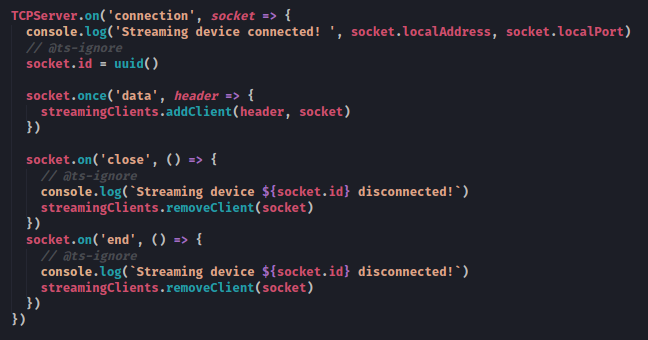
\includegraphics[width=\textwidth]{tcp_connections.png}
  \caption{Obrađivanje TCP konekcija}
\end{figure}

\begin{figure}
  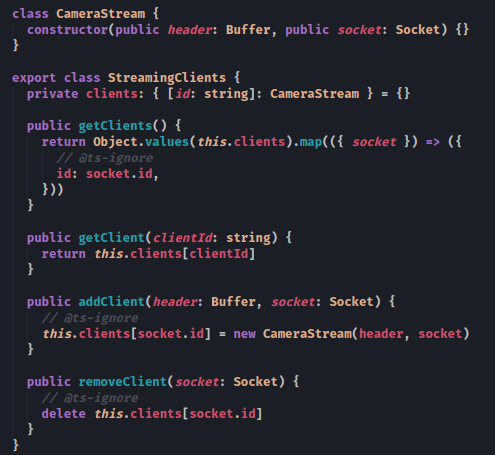
\includegraphics[width=\textwidth, height=10cm]{streaming_clients.png}
  \caption{Klase StreamingClients i CameraStream}
\end{figure}
\clearpage
\subsubsection{Prijenos klijentima}
Primarni način kojim poslužitelj komunicira s klijentima je HTTP (\foreign{Hypertext Transfer Protocol}) protokol.
\paraBreak
Ovaj protokol je temelj podatkovne komunikacije weba, baziran na zahtjev-odgovor principu gdje klijent primjerice
web preglednik šalje zahtjev nekom poslužitelju koji zauzvrat vrača odgovor u obliku HTML teksta, datoteke i ostalo.
\paraBreak
Format klijentskog zahtjeva se sastoji od rute koja predstavlja željeni resurs, primjerice '/korisnici', zaglavlja
zahtjeva, metoda, te opcionalno tijelo zahtjeva.
Metoda predstavlja tip akcije koji klijent želi odraditi, najbitnije od kojih su:
\begin{itemize}
  \item GET - dohvaćanje resursa, ne smije na nikakav način modificirati sam resurs
  \item POST - kreiranja novog resursa
  \item PUT - ažuriranje postojećeg resursa
  \item DELETE - brisanje resursa
\end{itemize}

\myparagraph{Rute} \label{sec:routes}
Na ovom poslužitelju postoje 4 glavne rute
\begin{itemize}
  \item [GET] /streams - vrača listu svih aktivnih kamera te njihove identifikatore, očekuje JWT token u zaglavlju
  \item [GET] /streams/:id/watch - vrača video podatke konkretne kamere ovisno o \\ 
    parametru \foreign{id} koji predstavlja identifikator kamere
  \item [POST] /auth/login - ruta za prijavu korisnika
  \item [GET] /auth/me - vrača podatke o korisniku dobivene iz tokena poslanog u zaglavlju
\end{itemize}
\noindent
Ruta \foreign{/watch} ne očekuje JWT token u zaglavlju jer zahtjev na ovu rutu u slučaju web preglednika vrši
\foreign{HTML5} video player nad kojim klijent nema kontrolu, zbog toga se token šalje kroz samu rutu u obliku
/watch?token='token'
\paraBreak
Sam proces slanja videa ove rute se odvija na sljedeći način:
\begin{enumerate}
  \item Verifikacija tokena iz rute
  \item Pronalaženje kamere po identifikatoru poslanom u ruti, u slučaju da kamera ne postoji poslužitelj odmah odgovara
    sa HHTP odgovorom 400 (engl. bad request)
  \item Postavljanje zaglavlja odgovora \foreign{Content-Type} na video/webm
  \item Zapisivanje zaglavlja videa iz dohvaćene kamere u odgovor
  \item Prosljeđivanje ostatka podataka iz kamere u odgovor
\end{enumerate}

\begin{figure}[h]
  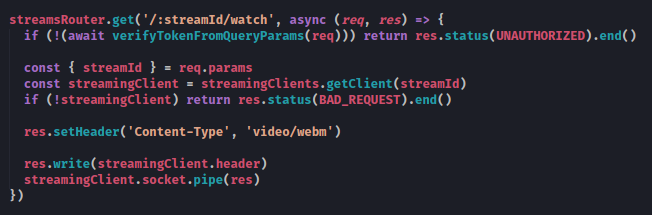
\includegraphics[width=\textwidth]{watch_endpoint.png}
  \caption{HTTP ruta za slanje videa}
  \label{pic:streaming}
\end{figure}
\noindent Nativna \foreign{Node js} funkcija pipe vidljiva na slici \ref{pic:streaming} može se pozvati nad bilo kojim tokom (engl. Stream) koji je tok čitanja
te joj se također prosljedi tok koji mora biti tok čitanja, rezltat ove funkcije je prijenos podataka iz jednog toka u
drugi.

\clearpage
\subsection{Web Klijent}
Web klijent implementiran kao dio ovog rada služi isključivo kao primjer, ideja je da se zbog izbora formata videa 
može jednostavno integrirati sa sustavom neovisno o platformi. \\
Sve što je potrebno za integraciju je video player koji podržava \foreign{webm} kontejner i \foreign{vp9} kodek.
\paraBreak
Sam klijent je vrlo jednostavan, sastoji se od forme za prijavu te prikaza svih trenutno spojenih kamera

\subsubsection{Autentifikacija}
Nakon što korisnik unese korisničko ime i lozinku šalje se zahtjev na poslužitelj koji u slučaju korektno poslanih
podataka odgovara s JWT tokenom \ref{sec:jwt}, zatim je korisnik preusmjeren na stranicu prikaza prijenosa.

\begin{figure} [h]
  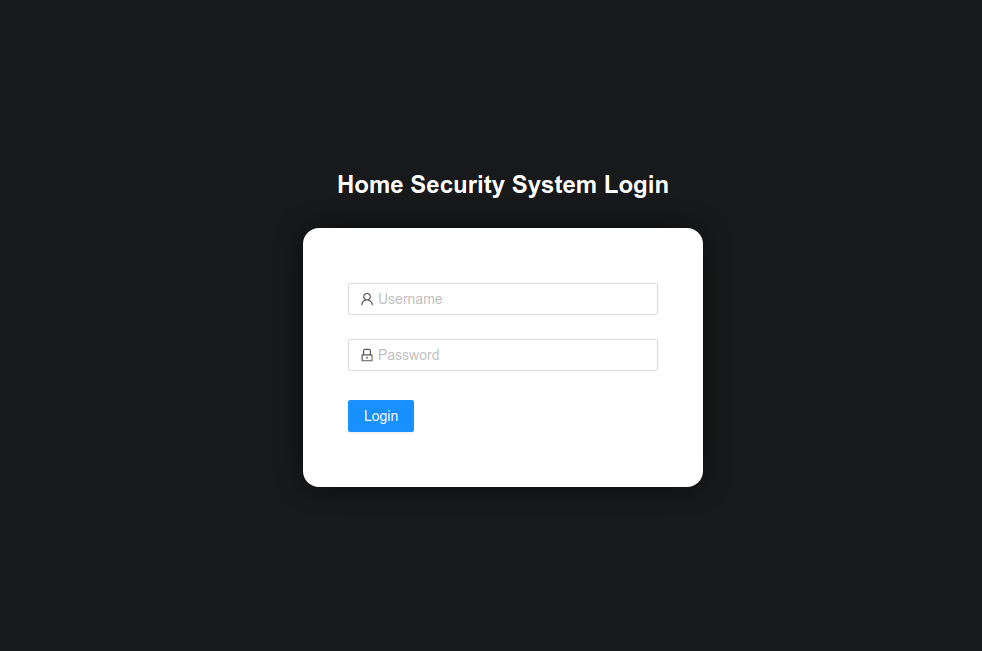
\includegraphics[width=\textwidth]{web_login.png}
  \caption{Forma za prijavu}
\end{figure}

\subsubsection{Prikaz živih prijenosa}
Prvi korak u prikazu prijenosa je zahtjev na poslužitelj za dohvat liste svih dostupnih kamera i njihovih identifikatora. 
Ovaj zahtjev očekuje \foreign{JWT} token u \foreign{Authorization} zaglavlju samog zahtjeva.
\\
Odgovor poslužitelja predstavlja popis svih kamera u obliku \foreign{array-a}, za svaku od kamera kreira se \foreign{HTML} 
video element kojem se izvor postavi na odgovarajuću rutu za gledanje \ref{sec:routes} ovisno o identifikatoru kamere

\begin{figure}[h]
  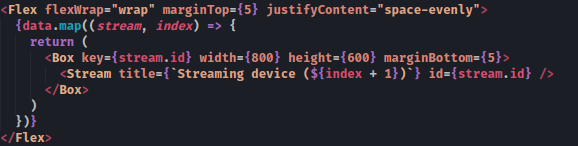
\includegraphics[width=\textwidth]{react_stream_list_comp.png}
  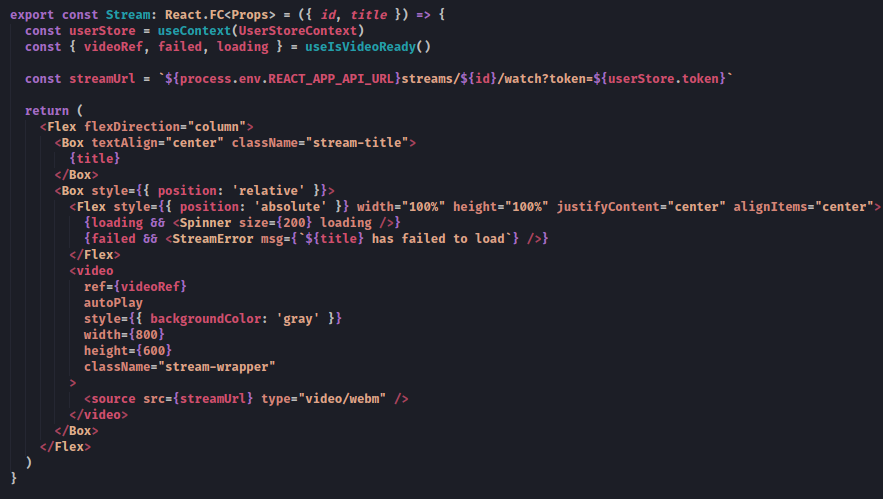
\includegraphics[width=\textwidth]{react_stream_comp.png}
  \caption{Implementacija u react-u}
\end{figure}

\begin{figure} [h]
  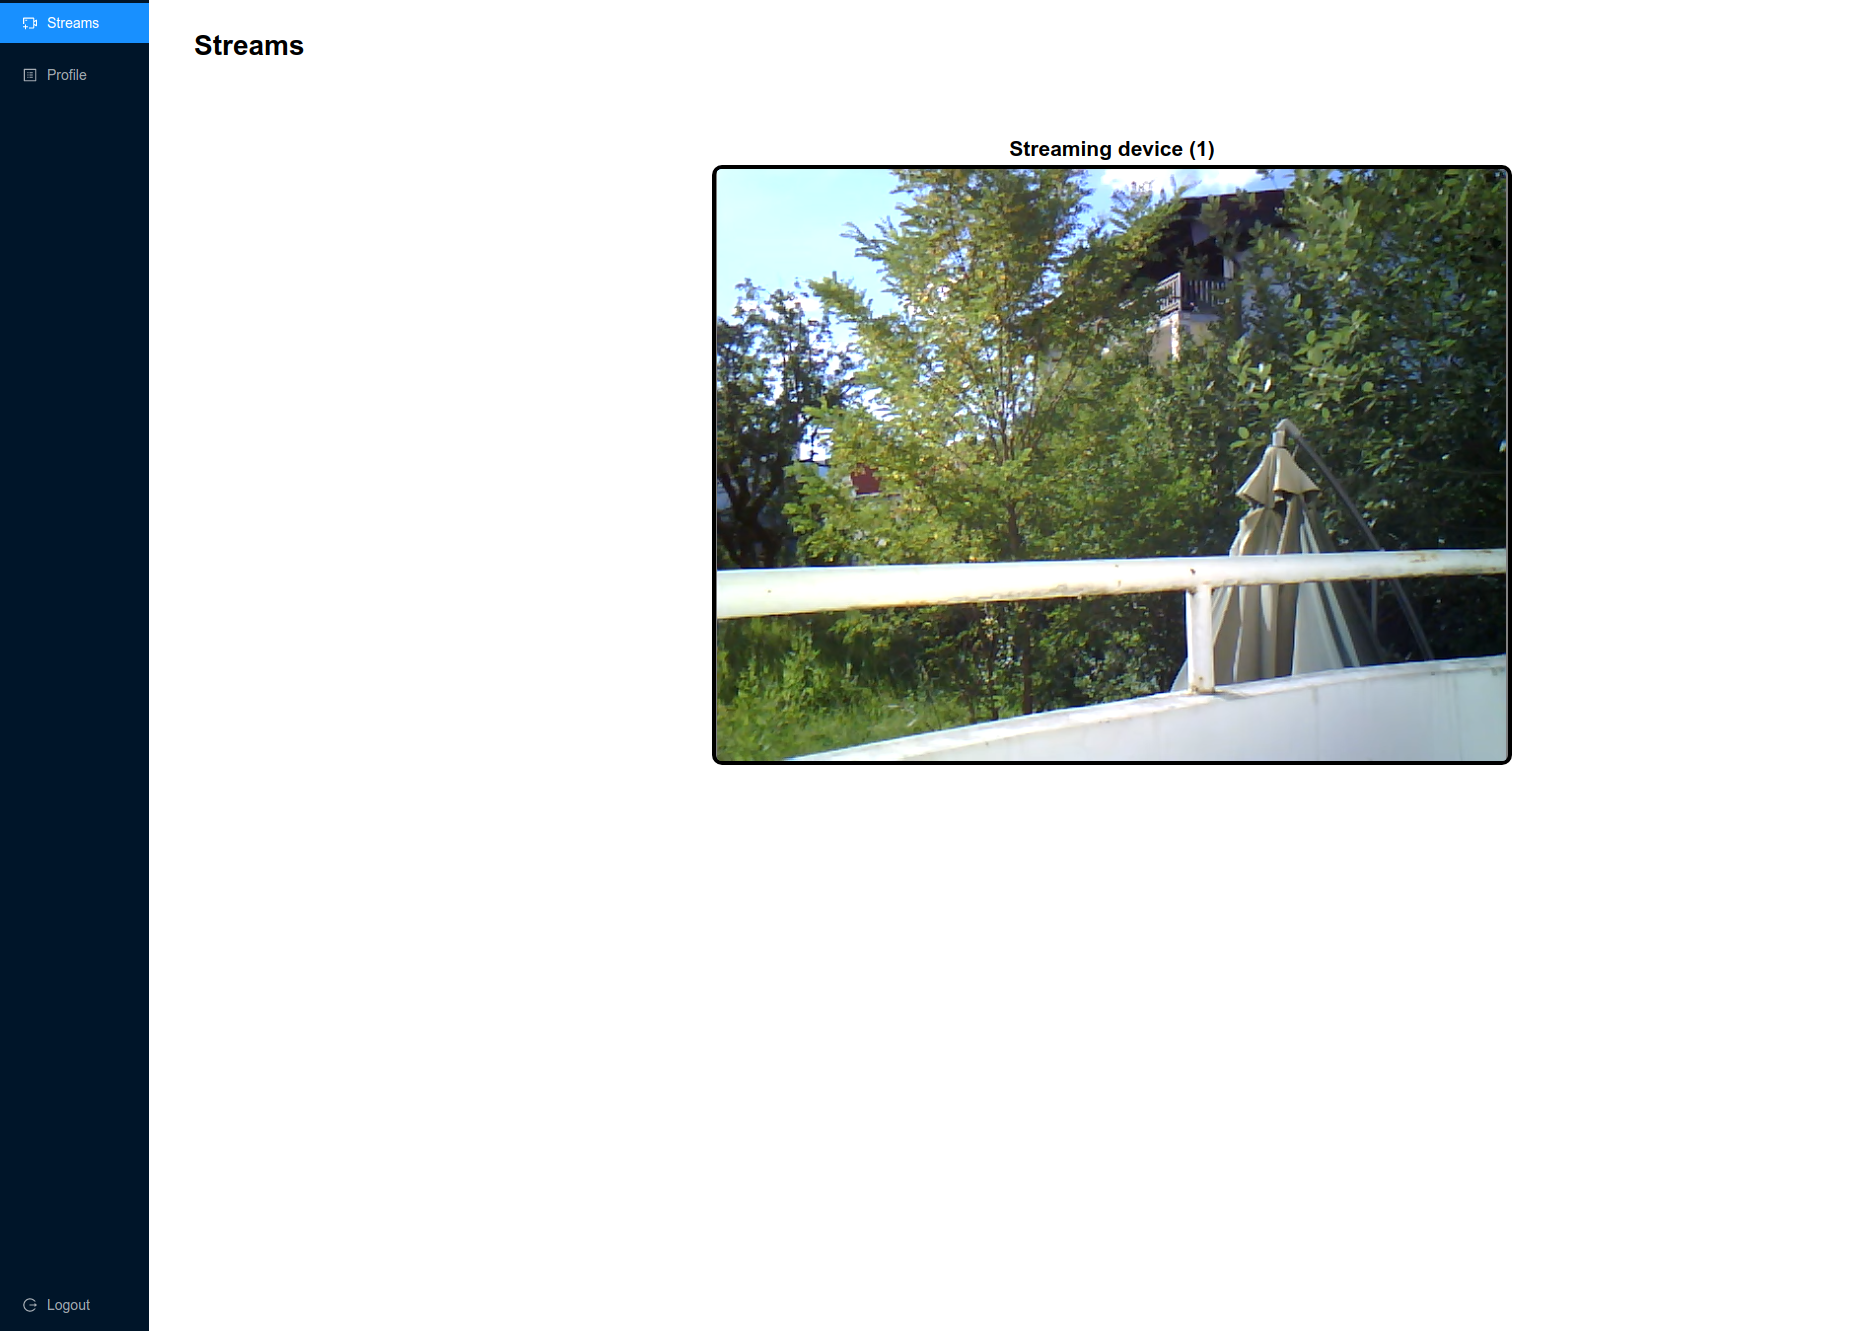
\includegraphics[width=\textwidth]{web_client1.png}
  \caption{Prikaz živih prijenosa}
\end{figure}

\begin{figure} [h]
  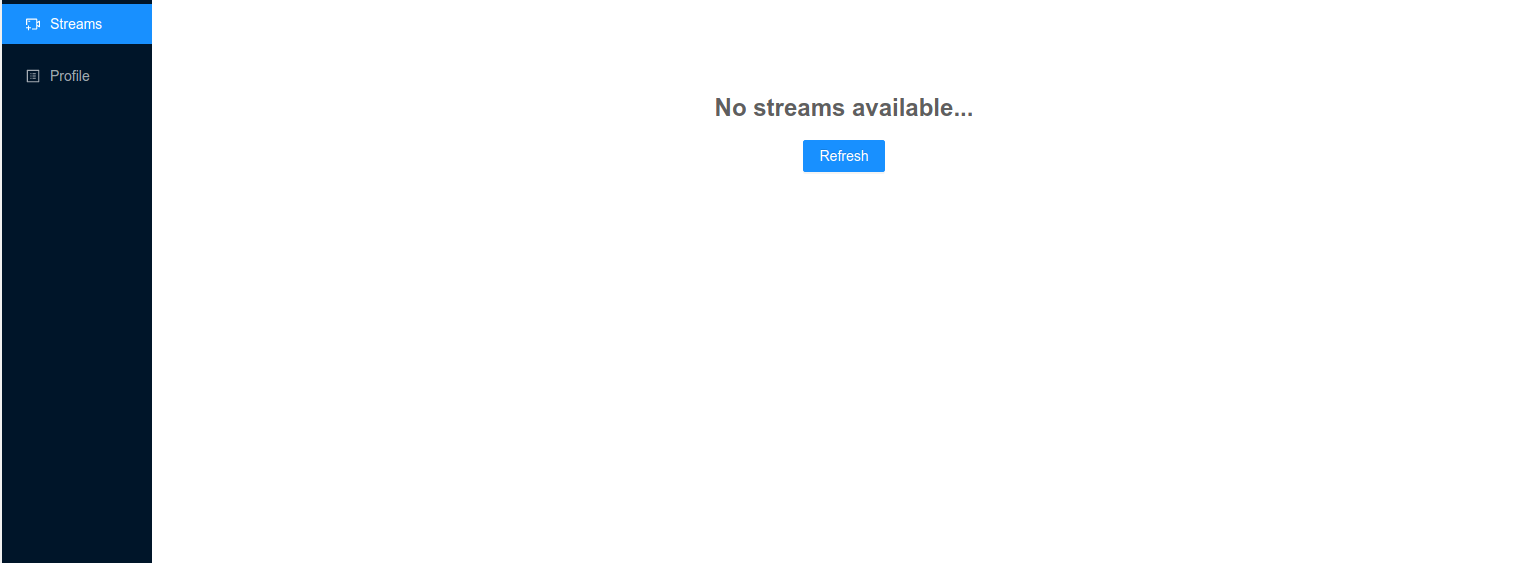
\includegraphics[width=\textwidth]{web_no_streams.png}
  \caption{Nema dostupnih prijenosa}
\end{figure}

\begin{figure} [h]
  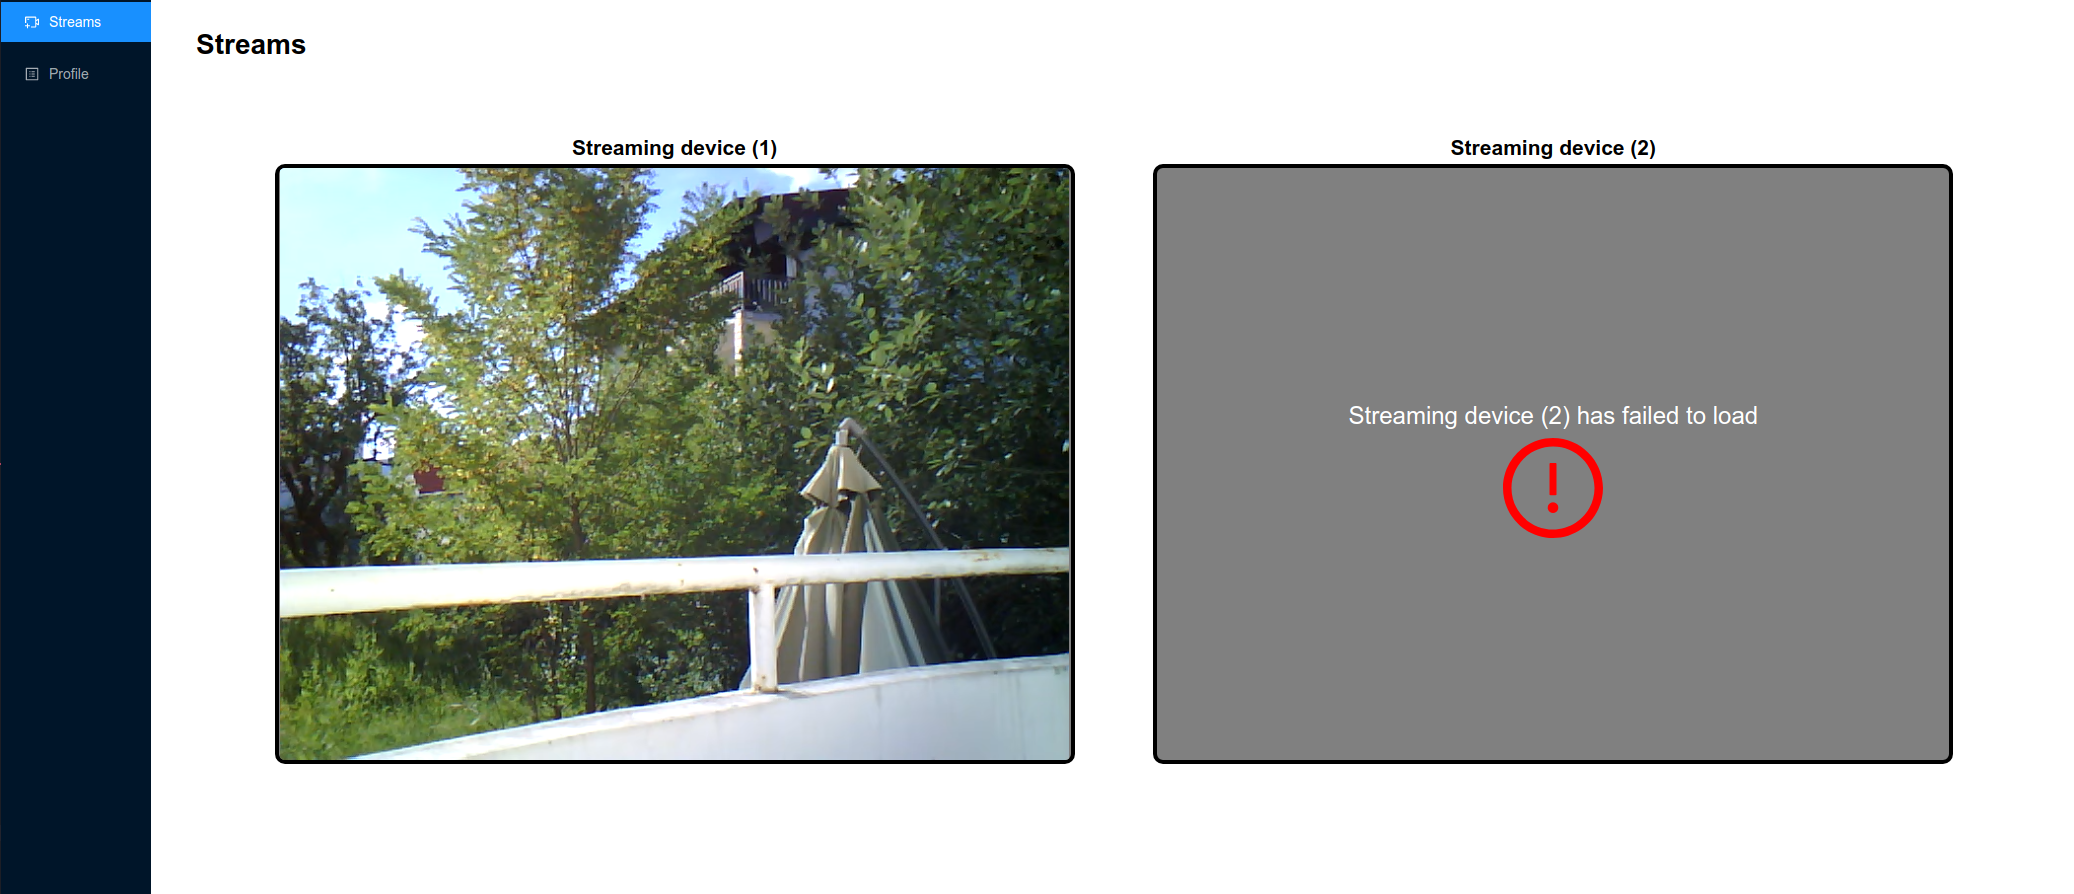
\includegraphics[width=\textwidth]{web_client_invalid_stream.png}
  \caption{Greška tijekom dohvaćanja živog prijenosa}
\end{figure}

\begin{figure} [h]
  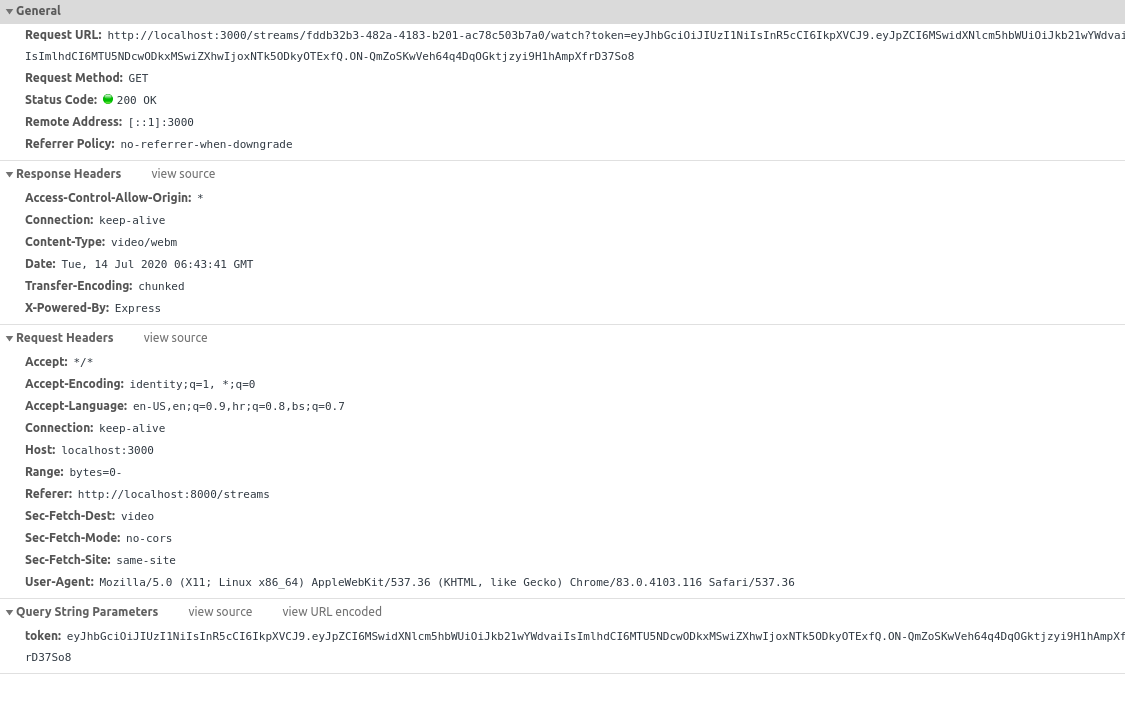
\includegraphics[width=\textwidth]{watch_request.png}
  \caption{Zahtjev za prijenos}
\end{figure}


\section{Zaključak}
Ovo je zaključak
\section{Literatura}

\begin{enumerate}
  \item Benjamin Binder, Computer Science Blog \\
  \url{https://blog.mi.hdm-stuttgart.de/index.php/2017/03/31/livestreaming-with-libav_-tutorial-part-1/}
  \item FFmpeg.org documentation \\
  \url{https://www.ffmpeg.org/doxygen/trunk/index.html}
  \item FFmpeg examples \\
  \url{https://code.videolan.org/libav/libav/-/tree/master/doc/examples}
  \item FFmpeg wiki, Streaming Guide \\
  \url{https://trac.ffmpeg.org/wiki/StreamingGuide}
  \item Node JS documentation  \\
  \url{https://nodejs.org/en/docs/}
  \item Flutter documentation \\
  \url{https://flutter.dev/docs}
  \item MDN \\
  \url{https://developer.mozilla.org/en-US/docs/Web/Media/Formats}
\end{enumerate}

\end{document}
